\documentclass[runningheads]{llncs}
%
\usepackage[utf8]{inputenc}
\usepackage{amsmath,amssymb}
\usepackage{graphicx}
\usepackage{booktabs}
\usepackage{tabularx}
\usepackage{algorithm}
\usepackage[noend]{algpseudocode}
\usepackage{xcolor}
\usepackage{tikz}
\usetikzlibrary{positioning,fit,arrows.meta,calc,backgrounds}
\usepackage[hidelinks]{hyperref}
\usepackage[expansion=false]{microtype}
%
% ---------------------------------------------------------------------------
% Screenshot helper: shows the image if it exists, otherwise a framed placeholder
% so the paper always compiles. Put screenshots in ./fig/
% ---------------------------------------------------------------------------
\usepackage{graphicx}
\usepackage{algpseudocode} % Cần thiết cho \algrenewcommand\algorithmicrequire...

\newlength{\shotw}
% Dùng \renewcommand nếu lệnh đã tồn tại ở class file, hoặc \newcommand nếu chưa có
\providecommand{\screenshot}[3]{% {file}{width}{placeholder text}
  \IfFileExists{#1}%
    {\includegraphics[width=#2]{#1}}%
    {%
      \setlength{\shotw}{#2}%
      \addtolength{\shotw}{-2\fboxsep}%
      \addtolength{\shotw}{-2\fboxrule}%
      \fbox{\parbox[c][0.5\shotw][c]{\shotw}{\centering\footnotesize\textit{Placeholder: #3}\\[2pt]\texttt{\detokenize{#1}}}}%
    }%
}

\newcommand{\code}[1]{\texttt{\detokenize{#1}}}
\newcommand{\Kb}{K_{\mathrm{best}}}
\algrenewcommand\algorithmicrequire{\textbf{Input:}}
\algrenewcommand\algorithmicensure{\textbf{Output:}}
\begin{document}
%
\title{An Explainable Human-in-the-Loop Framework for Temporal Video Event Retrieval using Z-Score Fusion and K-Best Monotonic Dynamic Programming}
\titlerunning{Explainable Human-in-the-Loop Temporal Video Retrieval}
%
\author{Ten-Tac-Gia-Chinh\inst{1}\orcidID{0000-0000-0000-0000} \and
Thanh-Binh Ngo-Viet\inst{1}\orcidID{0009-0001-0053-1499}}

\authorrunning{HoTacGiaChinh and Ngo-Viet}

\institute{University of Science, VNU-HCM, Ho Chi Minh City, Vietnam\\
\email{\{mssvbankia,24120269\}@student.hcmus.edu.vn}}
%
\maketitle
%
\begin{abstract}
We present an interactive system that answers Vietnamese queries over 873 news and broadcast videos (154,640 keyframes) for the three tasks of the Ho Chi Minh City AI Challenge 2026: known-item search, question answering, and temporal retrieval and alignment of key events (TRAKE). Its principle is that \emph{the machine brings the operator to the right region and the operator commits the answer}, so every AI component returns verifiable evidence rather than an opaque score. We contribute (i) a moment-level text index of 275,567 time-stamped ASR, OCR and metadata documents, matched by character trigrams with an $O(L)$ sliding-window containment test that tolerates OCR noise; (ii) a late fusion scheme that expresses all signals in units of the query's visual z-score; (iii) a K-Best Monotonic Dynamic Programming algorithm for chronological event alignment, which extends an $O(nK)$ monotonic-deque recurrence to the $\Kb$ best temporally distinct sequences using a max-heap with lazy deletion; and (iv) Deferred Diversity Reranking, a two-zone submission builder derived from the competition's rank-based scoring function.
\keywords{Interactive video retrieval \and Temporal alignment \and Dynamic programming \and Multi-modal fusion \and Human-in-the-loop.}
\end{abstract}
%
%============================================================================
\section{Introduction}
%============================================================================

Interactive video retrieval, shaped by benchmarks such as the Video Browser Showdown (VBS)~\cite{vadicamo2024vbs}, is dominated by vision--language embeddings such as SigLIP~\cite{zhai2023siglip}. The Ho Chi Minh City AI Challenge (AIC) is harder: queries are in Vietnamese, the decisive clue in news footage is often a spoken name or caption rather than a visual concept, and TRAKE requires localizing an \emph{ordered sequence} of semantic moments, each typically shorter than ten frames~\cite{do2025abstraction}.

This exposes three bottlenecks: OCR text is noisy and video-level BM25 tells \emph{which} video contains a term but not \emph{when}; rank fusion~\cite{cormack2009rrf,samuel2025mmmorrf} discards how strongly each signal matched; and alignment must run interactively while returning several plausible sequences, since visual scores are imperfect. A further factor is the scoring function itself, which averages the best of 100 submitted rows within the top $k\in\{1,5,20,50,100\}$; we argue that it, not generic heuristics, should dictate how the list is filled. Our contributions are:
\begin{enumerate}
\item a noise-tolerant \textbf{moment-level text index} (Sect.~\ref{sec:anchor});
\item \textbf{z-score late fusion}, giving all constants one interpretable unit (Sect.~\ref{sec:fusion});
\item a \textbf{K-Best Monotonic DP} with unlimited skipping, decoding the $\Kb$ best distinct alignments via a max-heap with lazy deletion (Sect.~\ref{sec:dp});
\item \textbf{Deferred MMR}, which keeps the top-20 slots rank-preserving and diversifies only the tail (Sect.~\ref{sec:mmr}).
\end{enumerate}

%============================================================================
\section{Related Work}
%============================================================================
VBS systems have converged on joint-embedding search with interactive browsing~\cite{vadicamo2024vbs,tran2025videoease}; recent AIC systems add LLM query expansion~\cite{vi2025heliosearch} and multi-modal fusion~\cite{nguyen2025vortex}, but often pass long descriptions to SigLIP, whose text encoder silently truncates beyond 64 tokens~\cite{zhai2023siglip}. For temporal alignment, DANTE~\cite{luu2025dante} applies a DP over keyframes, TARS~\cite{do2025tars} uses graph-based temporal search, VidAlign~\cite{nguyen2025vidalign} adds LLM co-searching, and KPT~\cite{vo2025kpt} targets Vietnamese news. Our DP differs in its state definition (indexed by the last \emph{matched} frame), its calibrated presence threshold, and its K-best decoding. Unlike RRF-based fusion~\cite{samuel2025mmmorrf}, we keep score margins, and unlike standard MMR~\cite{carbonell1998mmr}, we diversify only where the metric rewards it.

%============================================================================
\section{System Architecture}
%============================================================================
\begin{figure}[t]
\centering
\resizebox{\textwidth}{!}{%
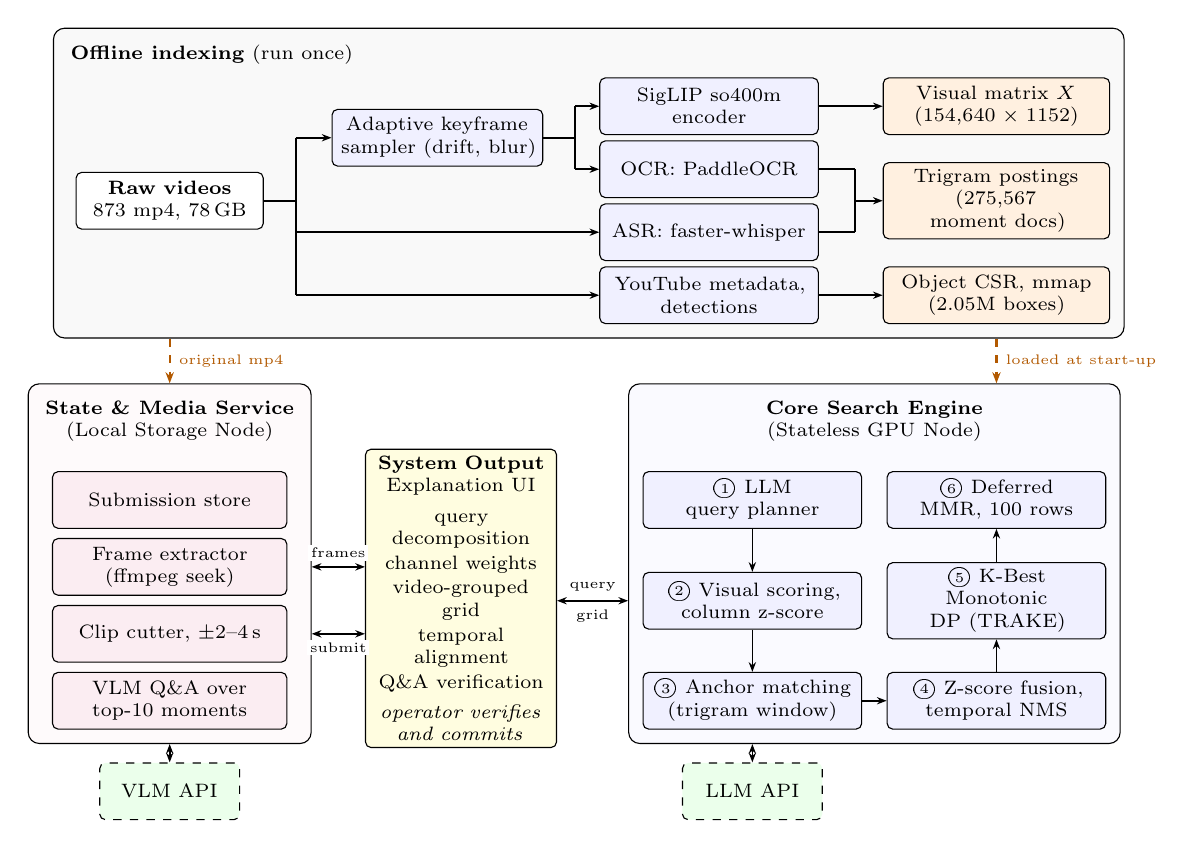
\begin{tikzpicture}[
  font=\scriptsize,
  every node/.append style={execute at begin node=\hyphenpenalty10000\exhyphenpenalty10000},
  box/.style={draw, rounded corners=2pt, align=center, fill=white, minimum height=0.72cm, inner sep=2.5pt, text width=#1},
  box/.default=2.4cm,
  proc/.style={box=#1, fill=blue!6}, proc/.default=2.6cm,
  art/.style={box=#1, fill=orange!12}, art/.default=2.7cm,
  st/.style={box=#1, fill=purple!7}, st/.default=2.8cm,
  ext/.style={box=#1, fill=green!8, dashed}, ext/.default=1.6cm,
  ttl/.style={align=center, font=\scriptsize, inner sep=1pt},
  grp/.style={draw, rounded corners=4pt, inner sep=5pt},
  arr/.style={-{Stealth[length=3.5pt]}, semithick},
  darr/.style={{Stealth[length=3.5pt]}-{Stealth[length=3.5pt]}, semithick},
  lbl/.style={font=\tiny, fill=white, inner sep=1pt},
  feed/.style={-{Stealth[length=4pt]}, dashed, orange!70!black, thick},
]
% ================= OFFLINE =================
\node[ttl, anchor=west] (offt) at (0.2,1.85) {\textbf{Offline indexing} (run once)};
\node[box=2.2cm] (vid) at (1.5,0.0) {\textbf{Raw videos}\\873 mp4, 78\,GB};
\node[proc=2.5cm] (kf) at (4.9,0.8) {Adaptive keyframe sampler (drift, blur)};
\node[proc] (sig) at (8.35,1.2) {SigLIP so400m encoder};
\node[proc] (ocr) at (8.35,0.4) {OCR: PaddleOCR};
\node[proc] (asr) at (8.35,-0.4) {ASR: faster-whisper};
\node[proc] (met) at (8.35,-1.2) {YouTube metadata, detections};
\node[art] (X) at (12.0,1.2) {Visual matrix $X$ ($154{,}640\times1152$)};
\node[art] (T) at (12.0,0.0) {Trigram postings (275,567 moment docs)};
\node[art] (O) at (12.0,-1.2) {Object CSR, mmap (2.05M boxes)};
\draw[semithick] (vid.east) -- (3.1,0.0);
\draw[semithick] (3.1,0.8) -- (3.1,-1.2);
\draw[arr] (3.1,0.8) -- (kf.west);
\draw[arr] (3.1,-0.4) -- (asr.west);
\draw[arr] (3.1,-1.2) -- (met.west);
\draw[semithick] (kf.east) -- (6.65,0.8);
\draw[semithick] (6.65,1.2) -- (6.65,0.4);
\draw[arr] (6.65,1.2) -- (sig.west);
\draw[arr] (6.65,0.4) -- (ocr.west);
\draw[arr] (sig) -- (X);
\draw[semithick] (ocr.east) -- (10.2,0.4);
\draw[semithick] (asr.east) -- (10.2,-0.4);
\draw[semithick] (10.2,0.4) -- (10.2,-0.4);
\draw[arr] (10.2,0.0) -- (T.west);
\draw[arr] (met.east) -- (O.west);
\begin{scope}[on background layer]
\node[grp, fill=gray!5, fit=(offt)(vid)(kf)(sig)(met)(X)(O)] (off) {};
\end{scope}
% ================= ONLINE =================
% state service (left)
\node[ttl] (stt) at (1.5,-2.8) {\textbf{State \& Media Service}\\(Local Storage Node)};
\node[st] (sub) at (1.5,-3.8) {Submission store};
\node[st] (fx) at (1.5,-4.65) {Frame extractor (ffmpeg seek)};
\node[st] (cl) at (1.5,-5.5) {Clip cutter, $\pm$2--4\,s};
\node[st] (qa) at (1.5,-6.35) {VLM Q\&A over top-10 moments};
\begin{scope}[on background layer]
\node[grp, fill=purple!2, fit=(stt)(sub)(qa)] (sts) {};
\end{scope}
% frontend (center)
\node[box=2.25cm, fill=yellow!12, minimum height=3.45cm] (fe) at (5.2,-5.05) {\textbf{System Output}\\Explanation UI\\[3pt]query decomposition\\[1pt]channel weights\\[1pt]video-grouped grid\\[1pt]temporal alignment\\[1pt]Q\&A verification\\[3pt]\textit{operator verifies and commits}};
% search service (right)
\node[ttl] (sst) at (10.45,-2.8) {\textbf{Core Search Engine}\\(Stateless GPU Node)};
\node[proc] (pl) at (8.9,-3.80) {\textcircled{\tiny 1} LLM query planner};
\node[proc] (vz) at (8.9,-5.08) {\textcircled{\tiny 2} Visual scoring, column z-score};
\node[proc] (am) at (8.9,-6.35) {\textcircled{\tiny 3} Anchor matching (trigram window)};
\node[proc] (fu) at (12.0,-6.35) {\textcircled{\tiny 4} Z-score fusion, temporal NMS};
\node[proc] (dp) at (12.0,-5.08) {\textcircled{\tiny 5} K-Best Monotonic DP (TRAKE)};
\node[proc] (mm) at (12.0,-3.80) {\textcircled{\tiny 6} Deferred MMR, 100 rows};
\draw[arr] (pl) -- (vz);
\draw[arr] (vz) -- (am);
\draw[arr] (am) -- (fu);
\draw[arr] (fu) -- (dp);
\draw[arr] (dp) -- (mm);
\begin{scope}[on background layer]
\node[grp, fill=blue!2, fit=(sst)(pl)(am)(fu)(mm)] (ss) {};
\end{scope}
% externals
\node[ext] (llm) at (8.9,-7.5) {LLM API};
\node[ext] (vlm) at (1.5,-7.5) {VLM API};
\draw[darr] (llm) -- (ss.south -| llm);
\draw[darr] (vlm) -- (sts.south -| vlm);
% offline -> online
\draw[feed] (off.south -| O) -- node[lbl, right=2pt]{loaded at start-up} (ss.north -| O);
\draw[feed] (off.south -| vid) -- node[lbl, right=2pt]{original mp4} (sts.north -| vid);
% frontend links
\draw[darr] (fe.east |- vz) -- node[lbl, above=2pt]{query} node[lbl, below=2pt]{grid} (ss.west |- vz);
\draw[darr] (fe.west |- fx) -- node[lbl, above=2pt]{frames} (sts.east |- fx);
\draw[darr] (fe.west |- cl) -- node[lbl, below=2pt]{submit} (sts.east |- cl);
\end{tikzpicture}%
}
\caption{System architecture. Offline, videos become a visual feature matrix, a moment-level trigram index and an object index. Online, a stateless GPU search service runs the numbered pipeline, while a state service on the competition machine holds submissions and serves frames, clips and VLM Q\&A directly from the original videos. The operator makes every final decision.}
\label{fig:arch}
\end{figure}

Figure~\ref{fig:arch} shows the architecture. The online part runs as three processes because the GPU search tier (FastAPI) may run elsewhere (e.g., a Kaggle instance tunnelled through ngrok), whereas the state tier (FastAPI + Socket.IO) must stay on the competition machine, which owns the submissions and the 78\,GB of videos; the frontend uses Next.js. A query passes through the numbered stages of Fig.~\ref{fig:arch}: a single structured-output LLM call produces a plan, all 154,640 keyframes are scored and fused, per-video temporal NMS forms \emph{moments}, TRAKE queries are aligned, and a 100-row list is built. The system never submits on its own.

\subsection{Offline Indexing}
\textbf{Keyframes.} A frame is kept when its cosine similarity to the last kept frame drops below a threshold in $[0.92,0.98]$ (spacing 0.5--5\,s); blurry frames below the video's 15th percentile of Laplacian variance are rejected. Each keyframe is embedded with SigLIP so400m-patch14-384~\cite{zhai2023siglip} (1152-d, L2-normalized).

\textbf{Moment-level text index.} With one BM25 document per video, long videos matched almost every query, and even the exact spoken sentence ranked the correct video only \#7--\#16; with one document per speech segment it ranked \#1. The index therefore attaches a timestamp to every document: 134,610 ASR documents (two consecutive faster-whisper large-v3~\cite{radford2023whisper} segments with $[t_0,t_1]$), 140,084 OCR documents (all PaddleOCR~\cite{du2020ppocr} text of one frame), and 873 metadata documents (YouTube title, description, keywords, author).

\textbf{Object index.} The organizers' detections from Faster R-CNN~\cite{ren2015faster} (177,321 keyframes, 2,054,901 boxes, 545 classes) are packed into a single 27\,MB CSR file that is memory-mapped, replacing 2.1\,GB of JSON.

\textbf{On-demand frames and clips.} Our keyframes differ from the organizers', so the exact frame to be submitted is decoded from the mp4 (about 88\,ms per ffmpeg seek, then cached). Clips of $\pm$2--4\,s distinguish ``walking in'' from ``walking out''; they are re-encoded because stream copy cuts only at codec keyframes.

%============================================================================
\section{Query Planning and Score Fusion}
%============================================================================
\subsection{LLM Query Plan}
\label{sec:plan}
The prompt follows each channel's limits: SigLIP understands only English and cannot read small text, so \code{visual_en} ($\le$55 words) describes visible content only, questions become statements, and Vietnamese concepts map to standard English terms (\textit{m\'ua l\^an} $\rightarrow$ ``lion dance''). The plan also contains \code{visual_short_en} ($\le$15 words, a guard against the 64-token limit), \code{events_en[]} for TRAKE, three anchor lists (\code{ocr_anchors}, \code{speech_anchors}, \code{meta_anchors}) and \code{question_vi}. It degrades in three tiers: full plan; translation with heuristic anchors; and, if translation fails, SigLIP is switched off, since Vietnamese input still yields plausible but meaningless cosines. Plans are cached on disk, so runs are deterministic.

\subsection{Visual Scoring with Per-Clause Z-Normalization}
Up to two strings, \code{visual_en} (weight 1.0) and \code{visual_short_en} (0.5), are encoded as $Q\in\mathbb{R}^{2\times1152}$ and scored exhaustively:
\begin{equation}
S=XQ^\top,\qquad Z=(S-\mu)\oslash\sigma,\qquad s_{\mathrm{vis}}=Zw\,/\textstyle\sum_j w_j,
\label{eq:vis}
\end{equation}
with $X\in\mathbb{R}^{154640\times1152}$ (float32, 712\,MB) and $\mu,\sigma$ taken per column, i.e., per query string. Each string has its own baseline (clause means from $-0.015$ to $+0.009$, standard deviations 0.024--0.033 within one query), so raw sums would favour the ``easy'' clause. A query costs about 0.36\,G multiply--accumulates, tens of milliseconds on a GPU, so approximate search would add error without meaningful speed-up.

\subsection{Anchor Matching with Trigrams and a Sliding Window}
\label{sec:anchor}
OCR in broadcasts loses diacritics and merges or drops characters (e.g., \textit{Vochong APhu}), so word matching fails. Each document is stripped of diacritics and spaces and hashed into character trigrams, stored as NumPy postings arrays. Matching has four steps.

\emph{Coarse filter:} postings are counted with \code{np.bincount}; a document survives if its matched fraction reaches 1.0 ($\le6$ trigrams), 0.85 ($\le12$) or 0.8 (longer). A short anchor missing one trigram is already another word. \emph{Fine filter:} containment ignores position (a transcript with ``ngu'' at the start and ``bang'' at the end contains every trigram of the name \textit{Ng\~u Bang}), so a window of $|\mathit{anchor}|+3$ characters slides over the document with two pointers and a frequency multiset, tracking the maximum number of distinct anchor trigrams inside it. Each position enters and leaves once, giving $O(L)$ time and a coverage $c\in[0,1]$. \emph{Rarity:} with $n$ matched documents and $k$ trigrams,
\begin{equation}
\mathit{info}=\frac{\log(\mathit{max\_hits}/n)}{\log\mathit{max\_hits}}\cdot\min\!\Big(1,\frac{k+2}{6}\Big),\qquad \mathit{max\_hits}=4000,
\label{eq:info}
\end{equation}
so ubiquitous anchors (``Viet Nam'') tend to zero, short anchors are down-weighted, and anchors with more than 4,000 hits are dropped. Anchors of at most four characters (``SIU'', ``HTV'') use a boundary-aware regular expression instead. \emph{Distribution:} each match adds $w=w_{\mathrm{channel}}\,c\,\mathit{info}$ to keyframes in $[t_0-\mathit{pad},t_1+\mathit{pad}]$ (3\,s ASR, 1.5\,s OCR) as the \emph{local} term and to all keyframes of its video as the \emph{video} term, at most one unit per anchor.

\subsection{Z-Score Late Fusion and Moment Formation}
\label{sec:fusion}
The fused keyframe score is
\begin{equation}
\mathit{score}=s_{\mathrm{vis}}+1.5\,a_{\mathrm{local}}+1.0\,a_{\mathrm{video}}.
\label{eq:fusion}
\end{equation}
We avoid RRF~\cite{cormack2009rrf} deliberately: ranks discard how strongly a signal matched, whereas the z-scale states that ``a local anchor is worth 1.5 standard deviations of visual evidence'', and all constants ($w_{\mathrm{local}}$, $w_{\mathrm{video}}$, $\tau$) share this unit. We also removed top-30 video pre-selection, which lost a correct video ranked \#31 among 400+ near-identical cooking videos. Finally, the top 6,000 frames are taken with \code{np.argpartition}, sorted, and scanned; a frame is dropped if the same video already has a kept frame within 0.5\,s. The system has no notion of shots, so all neighbourhoods are defined on \code{pts_time}.

%============================================================================
\section{K-Best Monotonic DP for Temporal Alignment}
\label{sec:dp}
%============================================================================
\subsection{Formulation and Recurrence}
A candidate video has keyframes at $t_1<\dots<t_n$, the query has $K$ ordered events, and $m_{i,k}$ is the calibrated score of frame $i$ for event $k$. We seek $i_1<\dots<i_K$ maximizing $\sum_k m_{i_k,k}$ subject to $\mathit{min\_gap}\le t_{i_{k+1}}-t_{i_k}\le\delta$ (defaults 0 and 30\,s); any event may be skipped at penalty $\gamma$, so videos missing an event remain comparable.

Let $dp[i][k]$ be the best score after the first $k$ events, where $i$ is the \emph{last matched} frame rather than the current frame. This is the crux: a skip does not advance the state, so several consecutive events can be skipped and the next match need only respect $\delta$ relative to the last frame actually used. The empty state is a separate scalar $\mathit{none}_k=-k\gamma$, from which a first match may start at any frame without the $\delta$ constraint:
\begin{equation}
dp[i][k]=\max\big\{\,m_{i,k}+\max_{j\in W(i)}dp[j][k-1],\ \ m_{i,k}+\mathit{none}_{k-1},\ \ dp[i][k-1]-\gamma\,\big\},
\label{eq:dp}
\end{equation}
i.e., match, first match, and skip, with $W(i)=\{j<i: t_i-\delta\le t_j\le t_i-\mathit{min\_gap}\}$ and $dp[\cdot][0]=-\infty$. The video score is $\max(\max_i dp[i][K],\mathit{none}_K)$. Because the skip branch forwards column $k-1$ into $k$, and $k$ forwards it into $k+1$, consecutive skips are unbounded and penalties accumulate. Since both ends of $W(i)$ move monotonically with $i$, a deque kept in decreasing order of $dp[j][k-1]$ yields each window maximum in amortized $O(1)$, reducing the naive $O(n^2K)$ loop to $O(nK)$.

\subsection{Calibration: the Presence Threshold $\tau$}
\label{sec:calib}
Raw cosines span only $[-0.064,0.135]$, so $\gamma=0.5$ exceeded any achievable match and skipping never happened. Per-event z-normalization fixed the scale but not the \emph{shape}: with a deliberately absent event (``a spacecraft landing on Mars''), $\gamma\in\{0,1,2,4,8\}$ gave identical outputs, because some frame always has positive $z$ and matching beats skipping whenever $z>-\gamma$. We therefore set $m_{i,k}=z_{i,k}-\tau$: a vaguely similar frame ($z=1$) becomes negative and is skipped, a true match ($z=3$) stays positive. With the 99th percentile of $z$ near 2.8 and the collection maximum near 3.8, $\tau=2.0$ is a sound boundary, and $\gamma$ becomes a structural penalty (default 0). The per-event $(\mu_k,\sigma_k)$ are estimated once per query from a stride-37 sample ($\approx$4,180 frames, 5\,ms) and shared by all videos; per-video estimates would make DP scores, which rank the candidate videos, incomparable.

\subsection{K-Best Extension with a Max-Heap and Lazy Deletion}
Since visual scores are noisy, the optimum of Eq.~\eqref{eq:dp} need not be the ground truth, and 99 more rows must be filled. Each state is therefore extended to a sorted list $D_k(i)$ of the $\Kb$ best partial solutions with back-pointers, and Eq.~\eqref{eq:dp} is applied to lists:
\begin{equation}
\begin{aligned}
D_k(i)=\operatorname{Top}_{\Kb}\Big(&\{m_{i,k}+v: v\in\operatorname{Top}_{\Kb}\textstyle\bigcup_{j\in W(i)}D_{k-1}(j)\}\\
&\cup\{m_{i,k}+\mathit{none}_{k-1}\}\cup\{v-\gamma: v\in D_{k-1}(i)\}\Big).
\end{aligned}
\label{eq:kbest}
\end{equation}
The inner term, the top-$\Kb$ values over the union of all lists in a sliding window, cannot be maintained by a monotonic deque, since each index now contributes $\Kb$ values. We keep a max-heap $H$ of entries $(v,j,r)$, the $r$-th value of $D_{k-1}(j)$. Entries are pushed when $j$ enters the window. A binary heap cannot delete arbitrary elements cheaply, so expired entries are removed \emph{lazily}: an entry is discarded when it reaches the top and $t_j<t_i-\delta$. This is exact because the left boundary is monotone, so an expired index never becomes valid again (Algorithm~\ref{alg:kbest}).

\begin{algorithm}[t]
\caption{K-Best Monotonic DP for one candidate video}
\label{alg:kbest}
\small
\begin{algorithmic}[1]
\Require times $t_{1..n}$, scores $m_{i,k}=z_{i,k}-\tau$, window $[\mathit{min\_gap},\delta]$, penalty $\gamma$, beam $\Kb$
\State $D_0(i)\gets\emptyset\ \forall i$;\quad $\mathit{none}_0\gets0$
\For{$k=1$ \textbf{to} $K$}
  \State $H\gets$ empty max-heap;\quad $p\gets1$ \Comment{next index to enter the window}
  \For{$i=1$ \textbf{to} $n$}
    \While{$p<i$ \textbf{and} $t_p\le t_i-\mathit{min\_gap}$} \Comment{right boundary}
      \State push all $(D_{k-1}(p)[r],p,r)$ into $H$;\quad $p\gets p+1$
    \EndWhile
    \State $A\gets[\,]$
    \While{$|A|<\Kb$ \textbf{and} $H\neq\emptyset$}
      \State $(v,j,r)\gets\textsc{Pop}(H)$; \textbf{if} $t_j<t_i-\delta$ \textbf{then continue} \Comment{lazy deletion}
      \State append $(v,j,r)$ to $A$
    \EndWhile
    \State push all entries of $A$ back into $H$
    \State $C\gets\{(m_{i,k}+v,\textsc{match},j,r)\}_{(v,j,r)\in A}\cup\{(m_{i,k}+\mathit{none}_{k-1},\textsc{first})\}$
    \State $C\gets C\cup\{(D_{k-1}(i)[r]-\gamma,\textsc{skip},i,r)\}_r$
    \State $D_k(i)\gets\operatorname{Top}_{\Kb}(C)$ \Comment{merge of sorted lists}
  \EndFor
  \State $\mathit{none}_k\gets\mathit{none}_{k-1}-\gamma$
\EndFor
\State \Return $\operatorname{Top}_{\Kb}\big(\bigcup_i D_K(i)\cup\{\mathit{none}_K\}\big)$
\end{algorithmic}
\end{algorithm}

\textbf{Complexity.} Each entry is pushed once on entry and discarded at most once; each query pops and re-pushes at most $\Kb$ valid entries. The heap holds at most $|W|_{\max}\Kb$ entries, where $|W|_{\max}\le\lceil\delta/\Delta t_{\min}\rceil+1=61$ is fixed by the sampling policy and independent of $n$. The total cost is therefore $O(n\,K\,\Kb\log(|W|_{\max}\Kb))=O(n\,K\,\Kb\log\Kb)$, which runs in real time on a CPU; for $\Kb=1$ the deque is used.

\textbf{Backtracking and deduplication.} Each entry stores its transition type and predecessor $(j,r)$, so each final entry traces back to a vector assigning every event a frame or ``skipped''; since match and skip branches merge at every event, alternatives differing in which events were skipped arise naturally. Distinct paths may, however, collapse to the same submission once skipped events are filled, so each completed frame tuple is inserted into a hash set and repeats are discarded; decoding from a slightly larger beam $\Kb'>\Kb$ guarantees exactly $\Kb$ temporally distinct sequences. They fill the TRAKE grid with principled alternatives rather than heuristic perturbations of one answer.

\textbf{Filling and local variants.} Submissions need one frame per event, so skipping only affects scoring: each skipped event later receives its most likely frame between its matched neighbours and is flagged \emph{weak}. After the operator confirms a sequence, variants are generated in increasing order of events changed (at most two alternatives per event), since the TRAKE R-score is the fraction of correct events and a 4/5 row can become 5/5 by moving only the misaligned event.

%============================================================================
\section{Deferred Diversity Reranking}
\label{sec:mmr}
%============================================================================
The competition score is $\mathit{Final}=\frac15\sum_{k\in\{1,5,20,50,100\}}R@k$. For KIS the R-score is binary, so $\mathit{Final}$ depends only on the rank $r$ of the first correct row: it equals $1.0$ for $r=1$, $0.8$ for $r\le5$, $0.6$ for $r\le20$, $0.4$ for $r\le50$, $0.2$ for $r\le100$, and 0 otherwise. Hence only the \emph{first} correct row counts, and slot values differ by up to $5\times$ across bands.

Diversifying all 100 rows with MMR~\cite{carbonell1998mmr} lowered our score. MMR measures redundancy visually, so alike frames from \emph{different} videos are penalized although, for the metric, they are not redundant; worse, the correct frame usually resembles the top-ranked one because it comes from the same shot, so it is penalized most. In two real queries, correct frames at ranks 9 and 11 (worth 0.6 each) were pushed out of the list entirely. Deferred MMR (Algorithm~\ref{alg:mmr}) uses two zones.

\textbf{Rank-preserving zone (rows 1--20).} No diversification is applied: moments appear strictly in order of the fused score (Eq.~\eqref{eq:fusion}), so a correct video that reaches the top keeps $R@1$, $R@5$ and $R@20$ intact. Around these moments the list is \emph{densified} with frames at a stride of 25 video frames, decoded from the mp4, to compensate for sparse keyframes relative to short ground-truth intervals.

\textbf{Diversity-injection zone (rows 21--100).} A greedy MMR with $\lambda=0.5$ fills the remaining rows, with redundancy defined \emph{temporally within a video} rather than visually. A candidate is penalized in inverse proportion to its temporal distance from moments already selected in the same video, and candidates from videos not yet listed receive no penalty:
\begin{equation}
c^\ast=\arg\max_{c\notin\mathcal{S}}\ \lambda\,\hat{s}(c)-(1-\lambda)\max_{u\in\mathcal{S},\,v(u)=v(c)}\min\!\Big(1,\frac{\Delta_0}{|t_c-t_u|}\Big),
\label{eq:mmr}
\end{equation}
where $\hat{s}$ is the fused score min--max normalized over the candidate pool, $v(\cdot)$ the video, $\Delta_0=8$\,s, and a maximum over the empty set is 0.

\begin{algorithm}[t]
\caption{Deferred MMR submission builder}
\label{alg:mmr}
\small
\begin{algorithmic}[1]
\Require moments $M$ sorted by fused score, boundary $R_0=20$, size $N=100$, $\lambda=0.5$, $\Delta_0$, stride $\rho=25$
\State $\mathcal{L}\gets[\,]$;\quad $\mathcal{S}\gets\emptyset$
\For{$c\in M$ \textbf{in order}} \Comment{zone 1: pure relevance}
  \State append $c$, then its densified neighbours at $\pm\rho,\pm2\rho,\dots$ frames, until $|\mathcal{L}|=R_0$
  \State $\mathcal{S}\gets\mathcal{S}\cup\{c\}$;\quad \textbf{if} $|\mathcal{L}|=R_0$ \textbf{then break}
\EndFor
\While{$|\mathcal{L}|<N$} \Comment{zone 2: temporal MMR, Eq.~\eqref{eq:mmr}}
  \State $c^\ast\gets\arg\max_{c\in M\setminus\mathcal{S}}\mathrm{MMR}(c\mid\mathcal{S})$;\quad append $c^\ast$ to $\mathcal{L}$;\quad $\mathcal{S}\gets\mathcal{S}\cup\{c^\ast\}$
\EndWhile
\State \Return $\mathcal{L}$
\end{algorithmic}
\end{algorithm}

The hybrid protects the first 20 slots, which carry 80\% of the attainable score, and spreads risk over the tail to recover $R@50$ and $R@100$ when the primary ranking misses.

%============================================================================
\section{Human-in-the-Loop Interaction}
%============================================================================
\textbf{Q\&A with a VLM.} The top 10 moments of the grid (same-video frames $<$4\,s apart) are sent to a VLM in parallel, each with its key frame and neighbours ($\le$3\,s) at 1280\,px, per-frame OCR and surrounding ASR. It returns \code{match}, \code{answerable}, \code{answer}, \code{evidence} and \code{best_frame}; \code{answerable} is true only if the answer is actually visible, readable or audible in that moment, not guessed or taken from outside knowledge. Identical answers are merged into votes; 1280\,px is kept because small-object counting failed at 896\,px.

\textbf{Specialized modes.} The operator can also search within results, draw class-and-count boxes on an object canvas (bridged to our keyframes via \code{pts_time}), and give Rocchio~\cite{rocchio1971} feedback in SigLIP space, $q'=\bar{x}_{+}-0.35\,\bar{x}_{-}$.

\textbf{Interface.} The main screen (Fig.~\ref{fig:ui}a) offers a three-state switch (\emph{Auto}, \emph{On}, \emph{Off}) per channel, coloured by the weight the channel actually contributes, and a status line showing the exact translation used. Result groups carry explanation tags (e.g., \emph{SigLIP: \#1}). The Q\&A panel (Fig.~\ref{fig:ui}b) shows votes and three-frame evidence; the TRAKE screen (Fig.~\ref{fig:ui}c) offers per-event $\pm12/\pm50$-frame nudges that preserve the order.

\begin{figure}[t]
\centering
\screenshot{fig/ui_main.png}{0.75\textwidth}{main search screen (Fig. 1 of the Vietnamese report)}\\[1pt]
{\footnotesize (a) Main screen: query, per-channel switches, video-grouped grid with explanation tags.}\\[4pt]
\begin{minipage}[t]{0.485\textwidth}\centering
\screenshot{fig/ui_qa.png}{\textwidth}{Q\&A panel}\\
{\footnotesize (b) Q\&A: merged answer with votes and three-frame evidence.}
\end{minipage}\hfill
\begin{minipage}[t]{0.485\textwidth}\centering
\screenshot{fig/ui_trake.png}{\textwidth}{TRAKE screen}\\
{\footnotesize (c) TRAKE: one row per event, per-event nudges.}
\end{minipage}
\caption{The interface shows every automatic decision together with its evidence.}
\label{fig:ui}
\end{figure}

%============================================================================
\section{Conclusion and Future Work}
%============================================================================
We presented an explainable, human-in-the-loop system for Vietnamese video event retrieval in which every component returns verifiable evidence. Deployed in the preliminary phase of the Ho Chi Minh City AI Challenge 2026 over 873 broadcast videos (78\,GB), the system achieved a cumulative score of 36.30 out of 86.00 evaluated points across three rounds (7.40, 18.70, and 10.20), for a Final Score of 0.618. The backend algorithms (z-score fusion, K-Best DP, Deferred MMR) ran without latency spikes or memory overflow throughout the competition.

Three lessons generalize: the unit of the text index matters more than the ranking model; a common, meaningful scale (the visual z-score) turns magic constants into tunable quantities, and its absence caused the two most serious DP failures; and optimization must follow the actual scoring function, which motivates both K-Best Monotonic DP for exploring optimal sequence variants, and Deferred MMR for diversifying the tail while strictly protecting the head of the list. Purely visual queries still depend entirely on SigLIP, and trigrams cannot recover ASR errors that transcribe a different sound. Future work includes segment-level video embeddings, a non-speech audio channel, unordered alignment for queries that merely list moments (an assignment problem solvable by the Hungarian algorithm in $O(K^3)$), and Vietnamese NER over ASR to mine anchors from the collection side.

\begin{credits}
\subsubsection{\ackname} The authors thank the organizers of the Ho Chi Minh City AI Challenge for providing the dataset and evaluation platform that inspired this work.

\subsubsection{\discintname}
The authors have no competing interests to declare that are relevant to the content of this article.
\end{credits}

%============================================================================
\begin{thebibliography}{99}
%============================================================================
\bibitem{carbonell1998mmr}
Carbonell, J., Goldstein, J.: The use of MMR, diversity-based reranking for reordering documents and producing summaries. In: Proc. 21st Annual International ACM SIGIR Conference, pp. 335--336 (1998)

\bibitem{cormack2009rrf}
Cormack, G.V., Clarke, C.L.A., B\"uttcher, S.: Reciprocal rank fusion outperforms Condorcet and individual rank learning methods. In: Proc. 32nd International ACM SIGIR Conference, pp. 758--759 (2009)

\bibitem{do2025tars}
Do, H.V., Do, Q.D., Nguyen, T.D., et al.: TARS: Temporal alignment retrieval system for efficient multi-segment video event retrieval. In: 14th International Symposium on Information and Communication Technology (SOICT). Springer (2025)

\bibitem{do2025abstraction}
Do, T.L., Huynh, V.T., Nguyen, H.D., et al.: Toward abstraction-level event retrieval in large video collections: Leveraging human knowledge and LLM-based reasoning in the Ho Chi Minh City AI Challenge 2025. In: 14th International Symposium on Information and Communication Technology (SOICT). Springer (2025)

\bibitem{du2020ppocr}
Du, Y., Li, C., Guo, R., et al.: PP-OCR: A practical ultra lightweight OCR system. arXiv preprint arXiv:2009.09941 (2020)

\bibitem{luu2025dante}
Luu, T.D., Nguyen-Dinh, L.V., Bui, D.B., et al.: Integrated semantic and temporal alignment for interactive video retrieval. In: 14th International Symposium on Information and Communication Technology (SOICT). Springer (2025)

\bibitem{nguyen2025vortex}
Nguyen, D.T., Tran-Minh, H.H., Lam, K.H., et al.: Vortex: Multi-modal fusion system for intelligent video retrieval. In: 14th International Symposium on Information and Communication Technology (SOICT). Springer (2025)

\bibitem{nguyen2025vidalign}
Nguyen, H.T., Tran, D.X., Vo, M.T., et al.: VidAlign: Integrating multi-event alignment and LLM co-searching for video retrieval. In: 14th International Symposium on Information and Communication Technology (SOICT). Springer (2025)

\bibitem{radford2023whisper}
Radford, A., Kim, J.W., Xu, T., Brockman, G., McLeavey, C., Sutskever, I.: Robust speech recognition via large-scale weak supervision. In: Proc. 40th International Conference on Machine Learning (ICML), pp. 28492--28518 (2023)

\bibitem{ren2015faster}
Ren, S., He, K., Girshick, R., Sun, J.: Faster R-CNN: Towards real-time object detection with region proposal networks. In: Advances in Neural Information Processing Systems (NeurIPS), vol.~28 (2015)

\bibitem{rocchio1971}
Rocchio, J.J.: Relevance feedback in information retrieval. In: Salton, G. (ed.) The SMART Retrieval System: Experiments in Automatic Document Processing, pp. 313--323. Prentice-Hall (1971)

\bibitem{samuel2025mmmorrf}
Samuel, S., DeGenaro, D., Yates, A., et al.: MMMORRF: Multimodal multilingual modularized reciprocal rank fusion. In: Proc. 48th International ACM SIGIR Conference on Research and Development in Information Retrieval (2025)

\bibitem{tran2025videoease}
Tran, Q.L., Nguyen, B., Jones, G.J.F., Gurrin, C.: VideoEase at VBS2025: An interactive video retrieval system. In: MultiMedia Modeling (MMM) (2025)

\bibitem{vadicamo2024vbs}
Vadicamo, L., Arnold, R., Bailer, W., Carrara, F., Gurrin, C., et al.: Evaluating performance and trends in interactive video retrieval: Insights from the 12th VBS competition. IEEE Access (2024)

\bibitem{vi2025heliosearch}
Vi, C.T., Luan, N.T., Nghi, T.G., et al.: HelioSearch: A multimodal video retrieval framework with LLM-driven query expansion and hybrid filtering. In: 14th International Symposium on Information and Communication Technology (SOICT). Springer (2025)

\bibitem{vo2025kpt}
Vo, T.P., Mai, D.K., et al.: KPT: Enhancing temporal event retrieval in Vietnamese news videos. In: 14th International Symposium on Information and Communication Technology (SOICT). Springer (2025)

\bibitem{zhai2023siglip}
Zhai, X., Mustafa, B., Kolesnikov, A., Beyer, L.: Sigmoid loss for language image pre-training. In: Proc. IEEE/CVF International Conference on Computer Vision (ICCV), pp. 11975--11986 (2023)
\end{thebibliography}
\end{document}